% =====================================================================
%  An Independent Statistical Audit of Adaptive Quantum Kernel Selection
%  for Clinical Cancer Diagnosis  --  Beamer presentation (37 slides)
%
%  Compile:  pdflatex audit_presentation.tex   (run twice so the outline
%            and section dividers are filled in)
%  Works on Overleaf with the default pdfLaTeX compiler.
% =====================================================================
\documentclass[aspectratio=169,11pt,t,xcolor={table}]{beamer}

% --- Speaker notes are written with \note{...}. They are hidden by default.
% --- To show them on a second screen, uncomment the next two lines:
% \usepackage{pgfpages}
% \setbeameroption{show notes on second screen=right}

\usetheme{Madrid}
\usepackage{amsmath,amssymb}
\usepackage{booktabs}
\usepackage{array}
\usepackage{graphicx}
\usepackage{tikz}
\usetikzlibrary{positioning,arrows.meta,calc,fit,backgrounds}
\usepackage{pgfplots}
\pgfplotsset{compat=1.18}
\usepackage{listings}

% ---------------------------------------------------------------------
%  Colours and theme
% ---------------------------------------------------------------------
\definecolor{qnavy}{HTML}{1B3A5C}
\definecolor{qteal}{HTML}{0E7C7B}
\definecolor{qred}{HTML}{B23A3A}
\definecolor{qgreen}{HTML}{2E7D4F}
\definecolor{qamber}{HTML}{C9821B}
\definecolor{qgray}{HTML}{6B7280}
\definecolor{qlight}{HTML}{EEF3F8}

\setbeamercolor{structure}{fg=qnavy}
\setbeamercolor{palette primary}{bg=qnavy,fg=white}
\setbeamercolor{palette secondary}{bg=qteal,fg=white}
\setbeamercolor{palette tertiary}{bg=qnavy,fg=white}
\setbeamercolor{palette quaternary}{bg=qnavy,fg=white}
\setbeamercolor{frametitle}{bg=qnavy,fg=white}
\setbeamercolor{title}{bg=qnavy,fg=white}
\setbeamercolor{subtitle}{fg=qlight}
\setbeamercolor{block title}{bg=qnavy,fg=white}
\setbeamercolor{block body}{bg=qlight,fg=black}
\setbeamercolor{block title alerted}{bg=qred,fg=white}
\setbeamercolor{block body alerted}{bg=qred!7,fg=black}
\setbeamercolor{block title example}{bg=qteal,fg=white}
\setbeamercolor{block body example}{bg=qteal!8,fg=black}
\setbeamercolor{item}{fg=qteal}
\setbeamercolor{alerted text}{fg=qred}
\setbeamercolor{simplebox}{bg=qamber!16,fg=black}
\setbeamercolor{tocbox}{bg=qlight,fg=black}
\setbeamercolor{author in head/foot}{bg=qnavy,fg=white}
\setbeamercolor{title in head/foot}{bg=qteal,fg=white}
\setbeamercolor{date in head/foot}{bg=qnavy,fg=white}
\setbeamercolor{section in toc}{fg=qnavy}

\setbeamertemplate{navigation symbols}{}
\setbeamertemplate{headline}{}
\setbeamertemplate{blocks}[rounded][shadow=false]
\setbeamertemplate{itemize item}[circle]
\setbeamertemplate{itemize subitem}[triangle]
\setbeamertemplate{enumerate items}[circle]
\setbeamertemplate{section in toc}{%
  \leavevmode{\color{qteal}\bfseries\MakeUppercase{\romannumeral\inserttocsectionnumber}.}~\inserttocsection\par}
\setbeamertemplate{section in toc shaded}[default][45]
\setbeamerfont{frametitle}{size=\large,series=\bfseries}
\newcolumntype{L}[1]{>{\raggedright\arraybackslash}p{#1}}
\newcommand{\tightdisplay}{\setlength{\abovedisplayskip}{2pt}\setlength{\belowdisplayskip}{2pt}%
  \setlength{\abovedisplayshortskip}{1pt}\setlength{\belowdisplayshortskip}{1pt}}
\setbeamerfont{block title}{size=\small,series=\bfseries}

% ---------------------------------------------------------------------
%  Helper macros
% ---------------------------------------------------------------------
% "In simple words" takeaway, pinned to the bottom of the slide
\newcommand{\insimple}[1]{%
  \par\vskip 0pt plus 1filll
  \begin{beamercolorbox}[wd=\textwidth,sep=4pt,rounded=true]{simplebox}%
    \small\textbf{\textcolor{qamber!75!black}{In simple words:}}\ #1%
  \end{beamercolorbox}\vskip1pt}

% Roman-numeral bubble for research questions
\newcommand{\qnum}[1]{\tikz[baseline=(n.base)]\node[circle,fill=qteal,text=white,
  font=\scriptsize\bfseries,inner sep=1pt,minimum size=6mm](n){#1};}

% Coloured verdict chip
\newcommand{\verdict}[2]{\tikz[baseline=(v.base)]\node[fill=#1!18,draw=#1,rounded corners=2pt,
  inner sep=2pt,font=\tiny\bfseries,text=#1!60!black](v){#2};}

% Guiding question shown on each section divider
\newcommand{\secquestion}{}

% Section divider slide
\AtBeginSection[]{%
\begin{frame}[c]
  \begin{columns}[c,onlytextwidth]
    \begin{column}{0.52\textwidth}
      {\color{qteal}\scalebox{2.4}{\Huge\bfseries\MakeUppercase{\romannumeral\insertsectionnumber}}}\par\vspace{5mm}
      {\LARGE\bfseries\color{qnavy}\insertsectionhead\par}\vspace{4mm}
      {\large\itshape\color{qgray}\secquestion\par}
    \end{column}
    \begin{column}{0.44\textwidth}
      \begin{beamercolorbox}[sep=8pt,rounded=true]{tocbox}
        \small\tableofcontents[currentsection,hideallsubsections]
      \end{beamercolorbox}
    \end{column}
  \end{columns}
\end{frame}}

% TikZ styles
\tikzset{
  >={Stealth[length=2mm]},
  flow/.style={draw=qnavy, fill=qlight, rounded corners=3pt, align=center,
               font=\scriptsize, minimum height=11mm, text width=18mm, inner sep=2pt},
  flowq/.style={flow, draw=qteal, fill=qteal!10},
  arr/.style={->, thick, draw=qnavy},
  mbox/.style={draw=qnavy, rounded corners=2pt, font=\scriptsize, minimum width=21mm,
               minimum height=5.6mm, inner sep=1pt},
}

% Code listing style
\lstdefinestyle{py}{language=Python,
  basicstyle=\ttfamily\fontsize{7}{8.4}\selectfont,
  keywordstyle=\color{qnavy}\bfseries, commentstyle=\color{qgray}\itshape,
  stringstyle=\color{qteal}, showstringspaces=false, columns=fullflexible,
  keepspaces=true, frame=single, rulecolor=\color{qgray!40},
  backgroundcolor=\color{qlight}, xleftmargin=3pt, xrightmargin=3pt,
  aboveskip=2pt, belowskip=0pt}

% ---------------------------------------------------------------------
%  Title information
% ---------------------------------------------------------------------
\title[Audit of Adaptive Quantum Kernel Selection]{An Independent Statistical Audit of Adaptive Quantum Kernel Selection for Clinical Cancer Diagnosis}
\subtitle{Multi-Seed Robustness, Familywise Error Control, and Cross-Dataset Generalization}
\author[Muhammad Wajahat]{Muhammad Wajahat, Member, IEEE}
\institute[]{Department of Computer Science\\National Biomedical Computational Center, Islamabad, Pakistan}
\date[October 2026]{October 2026}

\begin{document}

% =====================================================================
%  1. Title
% =====================================================================
\begin{frame}[c]
  \titlepage
  \note{Introduce yourself and the scope: this is an independent, code-level audit of one published quantum machine-learning framework for breast-cancer diagnosis (Daga et al., 2026), with a replication on a second dataset.}
\end{frame}

% =====================================================================
%  2. Outline
% =====================================================================
\begin{frame}{Outline}
  \begin{columns}[T,onlytextwidth]
    \begin{column}{0.52\textwidth}
      \tableofcontents[hideallsubsections]
    \end{column}
    \begin{column}{0.45\textwidth}
      \vspace{6mm}
      \begin{block}{What this talk does}
        A published paper says a quantum model diagnoses breast cancer better than a classical one. We re-run their code, test the claim more fairly, and repeat it on a second dataset.
      \end{block}
      \begin{exampleblock}{Datasets}
        WDBC ($N=569$, main audit) and WBCO ($N=683$, independent replication)
      \end{exampleblock}
    \end{column}
  \end{columns}
\end{frame}

% =====================================================================
%  3. Abbreviations
% =====================================================================
\begin{frame}{Abbreviations Used in This Talk}
  \footnotesize
  \setlength{\tabcolsep}{4pt}
  \renewcommand{\arraystretch}{1.1}
  \begin{columns}[T,onlytextwidth]
    \begin{column}{0.46\textwidth}
      \begin{tabular}{@{}>{\bfseries\color{qteal}}l L{49mm}@{}}
        \toprule
        QML  & Quantum Machine Learning \\
        NISQ & Noisy Intermediate-Scale Quantum \\
        SVM  & Support Vector Machine \\
        RBF  & Radial Basis Function (Gaussian) \\
        QSVM & Quantum Support Vector Machine \\
        QKNN & Quantum $k$-Nearest Neighbours \\
        OOF  & Out-of-Fold (stacking) \\
        HV   & Hard Voting (ensemble) \\
        PCA  & Principal Component Analysis \\
        IQP  & Instantaneous Quantum Polynomial \\
        RX/RZZ & X-rotation / ZZ entangling gates \\
        PSD  & Positive Semi-Definite \\
        FNA  & Fine-Needle Aspirate (biopsy) \\
        \bottomrule
      \end{tabular}
    \end{column}
    \begin{column}{0.52\textwidth}
      \begin{tabular}{@{}>{\bfseries\color{qteal}}l L{53mm}@{}}
        \toprule
        WDBC & Wisconsin Diagnostic Breast Cancer \\
        WBCO & Wisconsin Breast Cancer Original \\
        UCI  & UC Irvine Machine Learning Repository \\
        CV   & Cross-Validation \\
        FWER & Familywise Error Rate \\
        FDR  & False Discovery Rate \\
        MCC  & Matthews Correlation Coefficient \\
        ECE  & Expected Calibration Error \\
        TN/TP & True Negative / True Positive \\
        FP/FN & False Positive / False Negative \\
        Acc/Prec & Accuracy / Precision \\
        Rec/Spec & Recall / Specificity \\
        \bottomrule
      \end{tabular}
    \end{column}
  \end{columns}
\end{frame}

% =====================================================================
\renewcommand{\secquestion}{Why audit a quantum cancer-diagnosis claim?}
\section{Introduction}
% =====================================================================

\begin{frame}{Why This Matters: Breast-Cancer Diagnosis}
  \begin{columns}[T,onlytextwidth]
    \begin{column}{0.52\textwidth}
      \begin{itemize}\setlength{\itemsep}{5pt}
        \item More than \textbf{2.3 million} new breast-cancer cases every year {\scriptsize(Sung et al., 2021)}
        \item A computer model looks at cell measurements from a biopsy and says: \textbf{cancer} (malignant) or \textbf{not cancer} (benign)
        \item Many models already do this very well on WDBC and WBCO, two standard test datasets
        \item So when someone says ``our new model is better'', we must check that claim carefully
      \end{itemize}
    \end{column}
    \begin{column}{0.45\textwidth}
      \centering
      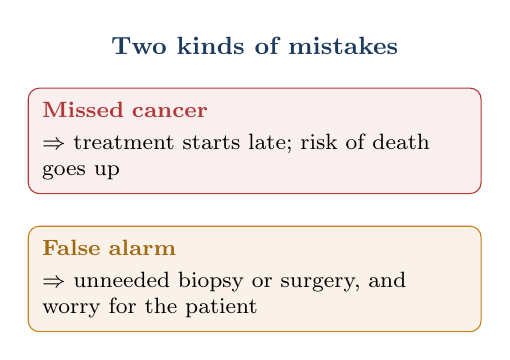
\begin{tikzpicture}[every node/.style={font=\footnotesize}]
        \node[font=\small\bfseries, text=qnavy] (h) {Two kinds of mistakes};
        \node[draw=qred, fill=qred!8, rounded corners=4pt, text width=54mm, align=left,
              inner sep=5pt, below=3mm of h] (fn)
          {\textbf{\color{qred}Missed cancer}\\[2pt]
           $\Rightarrow$ treatment starts late; risk of death goes up};
        \node[draw=qamber, fill=qamber!10, rounded corners=4pt, text width=54mm, align=left,
              inner sep=5pt, below=4mm of fn] (fp)
          {\textbf{\color{qamber!80!black}False alarm}\\[2pt]
           $\Rightarrow$ unneeded biopsy or surgery, and worry for the patient};
      \end{tikzpicture}
    \end{column}
  \end{columns}
  \insimple{In cancer diagnosis, a model's claim affects real patients, so it must be tested carefully.}
  \note{Start with the clinical stakes. A missed cancer delays treatment; a false alarm leads to unnecessary procedures. Because mistakes are costly, any claim that a new method is more accurate needs strong evidence.}
\end{frame}

\begin{frame}{What Is a Quantum Kernel?}
  \begin{itemize}\setlength{\itemsep}{3pt}
    \item Today's quantum computers are small and noisy (``\textbf{NISQ}'') {\scriptsize(Preskill, 2018)}; most research \textbf{simulates} them on normal computers
    \item A \textbf{kernel} measures how \emph{similar} two patients are; a \textbf{quantum kernel} does this with quantum states
    \item The big question: does quantum similarity give \emph{better} predictions than classical methods?
  \end{itemize}
  \vspace{3mm}
  \centering
  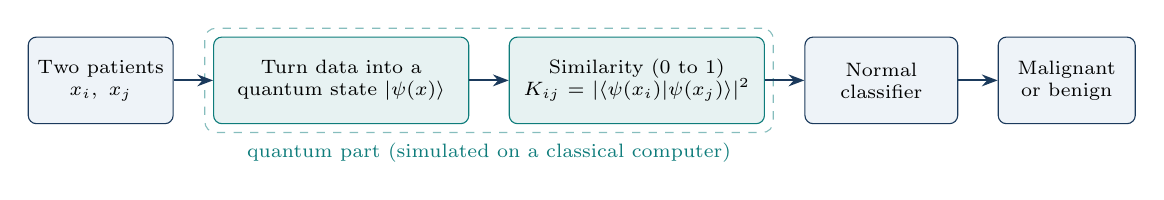
\begin{tikzpicture}[node distance=5mm]
    \node[flow, text width=17mm] (a) {Two patients\\$x_i,\ x_j$};
    \node[flowq, right=of a, text width=31mm] (b) {Turn data into a\\quantum state $|\psi(x)\rangle$};
    \node[flowq, right=of b, text width=31mm] (c) {Similarity (0 to 1)\\$K_{ij}=|\langle\psi(x_i)|\psi(x_j)\rangle|^2$};
    \node[flow, right=of c, text width=18mm] (d) {Normal\\classifier};
    \node[flow, right=of d, text width=16mm] (e) {Malignant\\or benign};
    \draw[arr] (a)--(b); \draw[arr] (b)--(c); \draw[arr] (c)--(d); \draw[arr] (d)--(e);
    \begin{scope}[on background layer]
      \node[fit=(b)(c), draw=qteal!50, dashed, rounded corners=4pt, inner sep=3pt,
            label={[font=\scriptsize, text=qteal]below:quantum part (simulated on a classical computer)}] {};
    \end{scope}
  \end{tikzpicture}
  \insimple{A quantum kernel is just a new way to measure ``how similar are two patients?''; the classifier on top is still a classical one.}
\end{frame}

\begin{frame}{The Claim We Checked: Daga et al.\ (2026)}
  \begin{columns}[T,onlytextwidth]
    \begin{column}{0.49\textwidth}
      \begin{block}{What they said}
        \footnotesize
        \begin{itemize}
          \item They built a \textbf{team of quantum models}: QSVM and QKNN, each with 3 kernel types (Angle, ZZ, Amplitude)
          \item A ``manager'' model combines the team (\textbf{stacking}); they called the choice of team members ``adaptive''
          \item They said it beats a normal classical model (\textbf{RBF-SVM}) in accuracy and when there is noise
          \item Tested on three clinical datasets: WDBC (breast cancer), Parkinson's and Diabetes
        \end{itemize}
      \end{block}
      {\scriptsize\color{qgray} Daga et al., \textit{Scientific Reports} 16, 26840 (2026)}
    \end{column}
    \begin{column}{0.48\textwidth}
      \begin{alertblock}{Why we checked it}
        \footnotesize
        \begin{itemize}
          \item Quantum ML results are often hard to repeat: random seeds, unclear data preparation, single runs
          \item A tool for cancer diagnosis needs very strong proof
          \item We \textbf{re-ran their own code} on WDBC and \textbf{repeated everything} on a second dataset (WBCO)
        \end{itemize}
      \end{alertblock}
    \end{column}
  \end{columns}
  \insimple{They said ``quantum beats classical''; we tested whether that is really true.}
  \note{Make clear that the audit is about one specific published framework and its released code. We do not claim anything about quantum computing in general.}
\end{frame}

% =====================================================================
\renewcommand{\secquestion}{What do we already know?}
\section{Literature Review}
% =====================================================================

\begin{frame}{What Earlier Research Tells Us}
  \begin{columns}[T,onlytextwidth]
    \begin{column}{0.53\textwidth}
      \begin{block}{About quantum kernels}
        \footnotesize
        \begin{itemize}
          \item \textbf{Havl\'{\i}\v{c}ek et al.\ (2019)}: first quantum kernels, including the ZZ map
          \item \textbf{Schuld \& Killoran (2019)}: a quantum model is really a kernel method --- the classifier on top is still classical
          \item \textbf{Liu et al.\ (2021)}: quantum wins are proven only for special, structured data; on ordinary data, classical kernels can be just as good
          \item \textbf{Tang (2019)}: some claimed quantum speed-ups can be copied by classical algorithms
        \end{itemize}
      \end{block}
    \end{column}
    \begin{column}{0.44\textwidth}
      \begin{block}{About fair testing}
        \footnotesize
        \begin{itemize}
          \item With 32 tests, at least one looks ``significant'' by pure luck \textbf{81\%} of the time ($1-0.95^{32}$)
          \item \textbf{Holm correction} (1979): makes the tests stricter so lucky wins are removed
          \item \textbf{Bootstrap} (Efron \& Tibshirani): re-sample the data many times to see how much results move
        \end{itemize}
      \end{block}
    \end{column}
  \end{columns}
  \insimple{Quantum wins are rare in theory, and many untested comparisons easily produce false wins.}
\end{frame}



% =====================================================================
\renewcommand{\secquestion}{What exactly is wrong, and what did we do about it?}
\section{Problem Statement and Contributions}
% =====================================================================

\begin{frame}{The Problem (1/2): How the Claim Was Tested}
  \small A wrong claim in cancer diagnosis can hurt patients. We found three weaknesses in \emph{how} the claim was tested:\par
  \vspace{3mm}
  \begin{columns}[T,onlytextwidth]
    \begin{column}{0.32\textwidth}
      \begin{block}{1 \textbullet{} Only one data split}
        \small
        All results come from \textbf{one} random split of the data (seed = 42).\\[4pt]
        \textbf{Why it matters:} one split can be lucky --- like judging a student on one exam.
      \end{block}
    \end{column}
    \begin{column}{0.32\textwidth}
      \begin{block}{2 \textbullet{} Many tests, no correction}
        \small
        8 models $\times$ 4 measures $=$ \textbf{32 tests}, with no correction for luck.\\[4pt]
        \textbf{Why it matters:} the chance of at least one false ``win'' is about \textbf{81\%}.
      \end{block}
    \end{column}
    \begin{column}{0.32\textwidth}
      \begin{block}{3 \textbullet{} Weak opponent}
        \small
        The classical model (RBF-SVM) kept its default settings ($C=1.0$, \texttt{gamma='scale'}) and was never tuned.\\[4pt]
        \textbf{Why it matters:} beating a weak opponent proves little.
      \end{block}
    \end{column}
  \end{columns}
  \insimple{The way it was tested made a quantum ``win'' easy to get by chance.}
  \note{Explain each weakness with the analogy. Seed 42 is one shuffle of the data. With 32 uncorrected tests, a false positive is almost guaranteed. Comparing against an untuned baseline tilts the field toward the new method.}
\end{frame}

\begin{frame}{The Problem (2/2): What the Code Really Does}
  \begin{columns}[T,onlytextwidth]
    \begin{column}{0.49\textwidth}
      \begin{block}{4 \textbullet{} The ``adaptive'' choice is fixed by hand}
        \small
        The paper says ``adaptive'' selection. In the code, the \textbf{same four} are always stacked: QSVM-Amplitude, QKNN-Amplitude, QSVM-ZZ, QKNN-Angle (chosen once by the authors for diversity).
        \textbf{QSVM-Angle}, the best quantum model in their own tables, is left out.\\[4pt]
        \textbf{Why it matters:} nothing is selected from the data inside the cross-validation.
      \end{block}
    \end{column}
    \begin{column}{0.49\textwidth}
      \begin{block}{5 \textbullet{} Noise test used different circuits}
        \small
        The noise simulation itself is done correctly (density matrices). But the noisy circuits are \textbf{not the ones benchmarked}: Angle uses $R_Y$ instead of $R_X$, and ZZ links only 7 neighbouring pairs instead of all 28 (\textbf{75\% fewer} entangling gates).\\[4pt]
        \textbf{Why it matters:} the ``robust to noise'' result is about a simpler, easier circuit.
      \end{block}
    \end{column}
  \end{columns}
  \insimple{Two main claims --- ``adaptive'' and ``robust to noise'' --- are not what the code actually does.}
  \note{These two problems were found by reading the released code, not only by re-running it. Be precise about noise: the released code uses PennyLane default.mixed (density matrices) and the trace stays exactly 1; the defect is that the noisy circuits differ from the clean benchmark circuits.}
\end{frame}

\begin{frame}{Our Three Questions}
  \vspace{3mm}
  \centering
  \renewcommand{\arraystretch}{1.7}
  \begin{tabular}{@{}c L{64mm} c L{54mm}@{}}
    & \textbf{Question} & & \textbf{How we answer it}\\
    \midrule
    \qnum{i}   & Is the quantum model \emph{really} better when we test on many splits and correct for luck? & $\Rightarrow$ & Re-run with 10 different splits; 32 tests with Holm correction \\
    \qnum{ii}  & Is the model choice really ``adaptive''? & $\Rightarrow$ & Read the code; let a fair automatic procedure choose \\
    \qnum{iii} & Do the findings hold on a second dataset? & $\Rightarrow$ & Repeat everything on WBCO (683 patients) \\
    \bottomrule
  \end{tabular}
  \insimple{Is it real? Is it adaptive? Does it hold on other data?}
\end{frame}



% =====================================================================
\renewcommand{\secquestion}{The data, the models, and how we test them}
\section{Audited Architecture and Methodology}
% =====================================================================

\begin{frame}{The Data: Two Breast-Cancer Datasets}
  \begin{columns}[T,onlytextwidth]
    \begin{column}{0.49\textwidth}
      \begin{block}{WDBC --- Wisconsin Diagnostic}
        \footnotesize
        \begin{itemize}
          \item \textbf{569 patients}: 212 cancer, 357 not cancer (37.3\% cancer)
          \item \textbf{30 measurements} of cell nuclei from a needle-biopsy (FNA) image: 10 properties, each as mean, standard error and worst value$^{\dagger}$
        \end{itemize}
        \vspace{1pt}{\scriptsize\color{qnavy}radius, texture, perimeter, area, smoothness, compactness, concavity, concave points, symmetry, fractal dimension\par}
      \end{block}
    \end{column}
    \begin{column}{0.49\textwidth}
      \begin{block}{WBCO --- Wisconsin Original}
        \footnotesize
        \begin{itemize}
          \item \textbf{683 patients} (16 with missing values removed): 239 cancer, 444 not cancer (35.0\% cancer)
          \item \textbf{9 cell features}, each given a score from 1 to 10$^{\dagger}$
        \end{itemize}
        \vspace{1pt}{\scriptsize\color{qnavy}clump thickness, uniformity of cell size, uniformity of cell shape, marginal adhesion, single epithelial cell size, bare nuclei, bland chromatin, normal nucleoli, mitoses\par}
      \end{block}
    \end{column}
  \end{columns}
  \vspace{1.5mm}
  \begin{beamercolorbox}[wd=\textwidth,sep=4pt,rounded=true]{block body alerted}
    \footnotesize\textbf{\color{qred}Important for reading the results:} in the code, 0 = cancer and 1 = not cancer.
    So \textbf{Recall} = how well non-cancer is recognised, and \textbf{Specificity} = how well cancer is found.
  \end{beamercolorbox}
  \vspace{1mm}
  {\tiny\color{qgray}$^{\dagger}$Feature names and descriptions: UCI Machine Learning Repository documentation; sample counts and dimensions ($D=30$, $D=9$) from the paper.\par}
  \insimple{Each row is one patient, each column is one cell measurement, and the answer is ``cancer'' or ``not cancer''.}
  \note{The label convention matters when reading the results tables: because benign is the "positive" class in the code, Specificity is the cancer-detection rate, and an FP is a malignant case predicted as benign.}
\end{frame}

\begin{frame}{How the Models Learn and Are Tested}
  \begin{columns}[T,onlytextwidth]
    \begin{column}{0.43\textwidth}
      \centering
      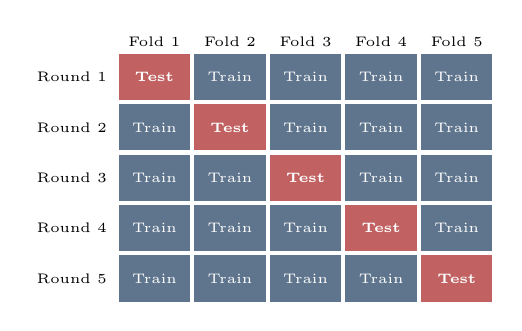
\begin{tikzpicture}[x=9.6mm,y=6.4mm]
        \foreach \cc in {1,...,5}{\node[font=\tiny] at (\cc,-0.3) {Fold \cc};}
        \foreach \rr in {1,...,5}{
          \node[font=\tiny, anchor=east] at (0.5,-\rr) {Round \rr};
          \foreach \cc in {1,...,5}{
            \ifnum\rr=\cc
              \node[draw=white, fill=qred!80, text=white, minimum width=9.2mm,
                    minimum height=6mm, font=\tiny\bfseries] at (\cc,-\rr) {Test};
            \else
              \node[draw=white, fill=qnavy!70, text=white, minimum width=9.2mm,
                    minimum height=6mm, font=\tiny] at (\cc,-\rr) {Train};
            \fi
          }
        }
      \end{tikzpicture}\par
      \vspace{1mm}
      {\scriptsize Cross-validation with 5 folds (example)}
    \end{column}
    \begin{column}{0.55\textwidth}
      \footnotesize
      \begin{itemize}\setlength{\itemsep}{3pt}
        \item The data are cut into equal parts (\textbf{folds}). The model learns on all parts but one and is tested on the part it has \textbf{not seen}
        \item Repeat until every patient has been tested \textbf{exactly once}
        \item Every fold keeps the same cancer / non-cancer mix (\textbf{stratified})
        \item Original study: one random cut (seed 42). \textbf{We}: 10 different random cuts
        \item The ``manager'' model (stacking) has its own inner 5-fold loop
      \end{itemize}
    \end{column}
  \end{columns}
  \insimple{Every patient is tested by a model that never learned from that patient --- and we reshuffle 10 times to rule out luck.}
  \note{Fig. 1 of the paper shows 10 outer stratified seeds and an inner 5-fold meta-CV for stacking. The global preprocessing in the released code comes from the project glossary and from Section V-D.}
\end{frame}

\begin{frame}{Preparing the Data (Same for Both Datasets)}
  \centering
  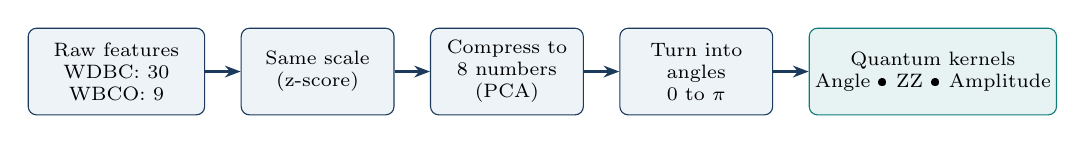
\begin{tikzpicture}[node distance=4.5mm]
    \node[flow, text width=21mm] (raw) {Raw features\\WDBC: 30 \quad WBCO: 9};
    \node[flow, right=of raw] (std) {Same scale\\(z-score)};
    \node[flow, right=of std] (pca) {Compress to\\8 numbers (PCA)};
    \node[flow, right=of pca] (mm) {Turn into angles\\$0$ to $\pi$};
    \node[flowq, right=of mm, text width=30mm] (q) {Quantum kernels\\Angle \textbullet\ ZZ \textbullet\ Amplitude};
    \draw[arr] (raw)--(std); \draw[arr] (std)--(pca); \draw[arr] (pca)--(mm); \draw[arr] (mm)--(q);
  \end{tikzpicture}\par
  \vspace{3mm}
  \begin{columns}[T,onlytextwidth]
    \begin{column}{0.30\textwidth}\centering
      {\footnotesize\bfseries Step 1: same scale}\par\vspace{1mm}
      $\displaystyle X^{(1)}=\frac{X-\mu}{\sigma}$\par{\scriptsize average 0, spread 1}
    \end{column}
    \begin{column}{0.30\textwidth}\centering
      {\footnotesize\bfseries Step 2: information kept}\par\vspace{1mm}
      $\displaystyle \mathrm{VR}(K)=\frac{\sum_{k=1}^{K}\lambda_k}{\sum_{j=1}^{D}\lambda_j}$\par{\scriptsize information kept by top 8}
    \end{column}
    \begin{column}{0.38\textwidth}\centering
      {\footnotesize\bfseries Step 3: into angles}\par\vspace{1mm}
      $\displaystyle X^{(3)}=\frac{X^{(2)}-X^{(2)}_{\min}}{X^{(2)}_{\max}-X^{(2)}_{\min}}\cdot\pi$\par{\scriptsize min $\to 0$, max $\to \pi$}
    \end{column}
  \end{columns}
  \vspace{3mm}
  \footnotesize
  \begin{itemize}
    \item 8 numbers keep \textbf{92.598\%} (WDBC) and \textbf{99.018\%} (WBCO) of the variation in the data
    \item 8 numbers $\rightarrow$ 8 qubits (Angle, ZZ), or 3 qubits for Amplitude (because $2^3=8$)
    \item Angles from 0 to $\pi$ are exactly the rotations a qubit gate can make
  \end{itemize}
  \insimple{Each patient becomes 8 numbers, and each number becomes a rotation angle for a qubit.}
\end{frame}

\begin{frame}{Three Ways to Measure Similarity (Quantum Kernels)}
  \centering
  \begin{beamercolorbox}[wd=0.78\textwidth,sep=4pt,rounded=true,center]{tocbox}
    $K(x_i,x_j)=|\langle\psi(x_i)|\psi(x_j)\rangle|^2$ \quad {\small = overlap of two quantum states (1 = same, 0 = different)}
  \end{beamercolorbox}
  \vspace{3mm}
  \begin{columns}[T,onlytextwidth]
    \begin{column}{0.32\textwidth}
      \begin{block}{Angle \hfill 8 qubits}
        \footnotesize
        Each number turns one qubit ($R_X$); qubits do not interact
        \[K=\prod_{k=1}^{n}\cos^2\!\Big(\frac{x_{ik}-x_{jk}}{2}\Big)\]
        Simple formula $\Rightarrow$ fast
      \end{block}
    \end{column}
    \begin{column}{0.32\textwidth}
      \begin{block}{ZZ (IQP-style) \hfill 8 qubits}
        \footnotesize
        Hadamards, $R_Z(x_k)$ on each qubit, then $R_{ZZ}$ gates that \textbf{link all 28 qubit pairs}
        \[\theta_{jk}=x_j\,x_k\]
        Qubits interact (entanglement)
      \end{block}
    \end{column}
    \begin{column}{0.32\textwidth}
      \begin{block}{Amplitude \hfill 3 qubits}
        \footnotesize
        The 8 numbers become the 8 amplitudes of 3 qubits
        \[K=\Big(\frac{x_i^{\top}x_j}{\|x_i\|\,\|x_j\|}\Big)^{2}\]
        Same as squared cosine similarity --- ordinary maths
      \end{block}
    \end{column}
  \end{columns}
  \insimple{Angle compares numbers one by one, ZZ also links every pair of qubits, and Amplitude is a classical similarity in disguise.}
  \note{All three formulas were checked against the cached Gram matrices: Angle and Amplitude closed forms match to about 1e-15, and the ZZ map is PennyLane IQPEmbedding (RZ(x) then ZZ(x_j x_k) on all pairs), also matching to about 1e-15.}
\end{frame}

\begin{frame}{The Models and How They Are Combined}
  \begin{columns}[T,onlytextwidth]
    \begin{column}{0.48\textwidth}
      \footnotesize\tightdisplay
      \textbf{QSVM} --- a normal SVM that uses the quantum similarity:
      \[\max_{\alpha}\ \sum_i\alpha_i-\tfrac12\sum_{i,j}\alpha_i\alpha_j y_i y_j K(x_i,x_j)\]
      \vspace{-1mm}\centerline{s.t.\ $0\le\alpha_i\le C$,\ \ $\sum_i\alpha_i y_i=0$}\vspace{1.5mm}
      \textbf{QKNN} --- find the 5 most similar patients and take a majority vote:
      \[D_Q(x_i,x_j)=\max\big(0,\,1-K(x_i,x_j)\big)\]
      \textbf{Stacking} --- a ``manager'' (logistic regression) weighs the 4 models' 0/1 answers:
      \[\hat p_i=\sigma\Big(\beta_0+\textstyle\sum_{m=1}^{4}\beta_m\,\hat c^{(oof)}_{im}\Big)\]
    \end{column}
    \begin{column}{0.50\textwidth}
      \centering
      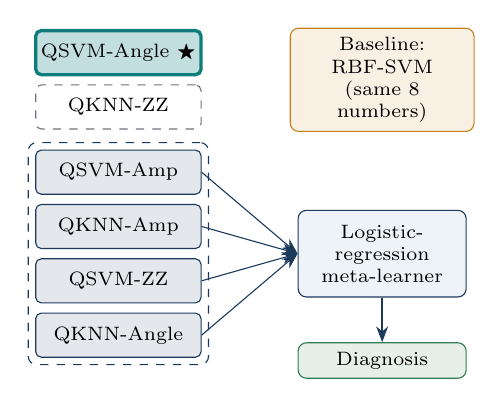
\begin{tikzpicture}[yscale=0.92]
        \node[mbox, fill=qteal!25, draw=qteal, very thick] (qa) at (0,0) {QSVM-Angle $\bigstar$};
        \node[mbox, fill=white, draw=qgray, dashed] (kz) at (0,-0.75) {QKNN-ZZ};
        \node[mbox, fill=qnavy!12] (qm) at (0,-1.65) {QSVM-Amp};
        \node[mbox, fill=qnavy!12] (km) at (0,-2.4) {QKNN-Amp};
        \node[mbox, fill=qnavy!12] (qz) at (0,-3.15) {QSVM-ZZ};
        \node[mbox, fill=qnavy!12] (ka) at (0,-3.9) {QKNN-Angle};
        \node[fit=(qm)(ka), draw=qnavy, dashed, rounded corners=3pt, inner sep=2.5pt] (quart) {};
        \node[draw=qnavy, fill=qlight, rounded corners=3pt, text width=19mm, align=center,
              font=\scriptsize, minimum height=11mm] (meta) at (3.35,-2.775) {Logistic-regression\\meta-learner};
        \node[draw=qgreen, fill=qgreen!12, rounded corners=3pt, font=\scriptsize,
              text width=19mm, align=center] (pred) at (3.35,-4.25) {Diagnosis};
        \foreach \m in {qm,km,qz,ka} \draw[->, qnavy] (\m.east) -- (meta.west);
        \draw[arr] (meta) -- (pred);
        \node[draw=qamber, fill=qamber!12, rounded corners=3pt, font=\scriptsize,
              text width=21mm, align=center] at (3.35,-0.375) {Baseline: RBF-SVM\\(same 8 numbers)};
      \end{tikzpicture}\par
      \vspace{1mm}
      {\tiny \textcolor{qnavy}{\textbf{Dashed box}}: published stacking quartet (hardcoded).\ $\bigstar$ strongest single quantum model --- not in it.\ Hard voting: majority of QSVM-ZZ, QKNN-Amp, QSVM-Angle.\par}
    \end{column}
  \end{columns}
  \insimple{Several ``expert'' models give an answer, and a ``manager'' learns how much to trust each expert.}
  \note{The released code stacks exactly four models (QSVM-Amp, QKNN-Amp, QSVM-ZZ, QKNN-Angle), and the meta-learner is trained on their inner-CV 0/1 predictions, not on probabilities. QSVM-Angle and QKNN-ZZ are not stacked; QSVM-Angle is used only in hard voting. This matches Eq. (11) and Fig. 1 of the v3 paper.}
\end{frame}

\begin{frame}{Our Statistical Tools in Plain Words}
  \begin{columns}[T,onlytextwidth]
    \begin{column}{0.49\textwidth}
      \begin{block}{Bootstrap: could it be luck?}
        \footnotesize\tightdisplay
        \[\hat p=\frac{2\,\big(1+\min(n_{\le 0},\,n_{\ge 0})\big)}{B+1}\]
        Re-sample the patients $B=10{,}000$ times; $n_{\le0}$ / $n_{\ge0}$ count how often the quantum$-$RBF gap is $\le 0$ / $\ge 0$. If the gap rarely changes sign, $p$ is small.
      \end{block}
    \end{column}
    \begin{column}{0.49\textwidth}
      \begin{block}{Holm correction: no lucky wins}
        \footnotesize
        Sort the 32 $p$-values. Accept a result only while $p_{(i)}\le\dfrac{0.05}{32-i+1}$; stop at the first failure.
        So the best result must beat $0.05/32\approx0.0016$.
      \end{block}
      \begin{block}{MCC: one fair score}
        \footnotesize\tightdisplay
        \[\mathrm{MCC}=\frac{TP\cdot TN-FP\cdot FN}{\sqrt{(TP{+}FP)(TP{+}FN)(TN{+}FP)(TN{+}FN)}}\]
        Uses all four boxes of the confusion matrix: $+1$ = perfect, $0$ = guessing, $-1$ = always wrong.
      \end{block}
    \end{column}
  \end{columns}
  \insimple{Bootstrap asks ``is it luck?'', Holm removes lucky wins, and MCC gives one fair score.}
\end{frame}

\begin{frame}[fragile]{How It Is Built in Code (Python)}
  \begin{columns}[T,onlytextwidth]
    \begin{column}{0.36\textwidth}
      \scriptsize
      \begin{itemize}\setlength{\itemsep}{3pt}
        \item \textbf{PennyLane} builds the quantum circuits and kernels
        \item \textbf{scikit-learn} does the scaling, PCA, the SVM and the ``manager''
        \item Two simulators in their code: \texttt{lightning.qubit} (statevectors, clean kernels) and \texttt{default.mixed} (density matrices, noise test)
        \item Their run: seed 42; Angle kernel from its simple formula
        \item Our audit: 10 seeds; 10,000 bootstrap re-samples
      \end{itemize}
    \end{column}
    \begin{column}{0.62\textwidth}
      {\scriptsize\bfseries\color{qred}Illustrative sketch -- not the released code}
\begin{lstlisting}[style=py]
import numpy as np
from sklearn.pipeline import make_pipeline
from sklearn.preprocessing import StandardScaler, MinMaxScaler
from sklearn.decomposition import PCA
from sklearn.svm import SVC
from sklearn.linear_model import LogisticRegression
prep = make_pipeline(StandardScaler(), PCA(n_components=8),
                     MinMaxScaler(feature_range=(0, np.pi)))
Z = prep.fit_transform(X_train)        # 8 angles per patient
def angle_kernel(A, B):                # closed form, Eq. (6)
    d = A[:, None, :] - B[None, :, :]
    return np.prod(np.cos(d / 2) ** 2, axis=2)
K = angle_kernel(Z, Z)                 # quantum Gram matrix
qsvm = SVC(kernel="precomputed").fit(K, y_train)
meta = LogisticRegression(class_weight="balanced"
          ).fit(C_oof, y_train)        # OOF 0/1 preds
\end{lstlisting}
    \end{column}
  \end{columns}
  \insimple{It is normal Python machine-learning code; only the similarity part is quantum.}
  \note{The tool and simulator names come from the paper and the project glossary. The listing is a teaching sketch of the described pipeline, not a copy of the released repository.}
\end{frame}

\begin{frame}{Our Audit Plan: Their Approach vs.\ Ours}
  \centering\footnotesize
  \renewcommand{\arraystretch}{1.15}
  \begin{tabular}{@{}L{48mm}c L{82mm}@{}}
    \toprule
    \textbf{What they did} & & \textbf{What we did}\\
    \midrule
    Tested on one split (seed 42)         & $\rightarrow$ & \textbf{0.} Get their exact numbers again; \textbf{1.} repeat with 10 splits (seeds 0--5, 10, 42, 100, 999) \\
    32 comparisons, no correction         & $\rightarrow$ & \textbf{2.} Bootstrap + Holm correction on all 32 tests \\
    Same four models always used          & $\rightarrow$ & \textbf{3.} Let a fair procedure pick 4 of 6 models (all 15 options, 3 rules) \\
    Noise test on simplified circuits     & $\rightarrow$ & \textbf{4.} Read the noise code; re-run it with the benchmarked circuits \\
    Default classical model; one dataset  & $\rightarrow$ & \textbf{5.} Tune the classical model; check the VQC gradients; repeat on WBCO \\
    \bottomrule
  \end{tabular}\par
  \vspace{1.5mm}
  {\scriptsize\color{qteal}\textbf{Reading guide:} Results 1--5 follow steps 0--3; Results 6--8 cover noise, the code checks and probabilities; Result 9 is the second-dataset check.\par}
  \insimple{We kept their method and only made the testing fair --- one check for each weakness.}
  \note{This slide is the bridge between methods and results: every weakness from Section III has a matching audit tier, and the results slides follow the same numbering.}
\end{frame}

% =====================================================================
\renewcommand{\secquestion}{What did the numbers actually show?}
\section{Empirical Results}
% =====================================================================

\begin{frame}{Result 1 --- Can We Get Their Numbers? (Seed 42)}
  \begin{columns}[T,onlytextwidth]
    \begin{column}{0.41\textwidth}
      \centering
      {\footnotesize\bfseries Classical RBF-SVM, WDBC, seed 42}\par\vspace{1mm}
      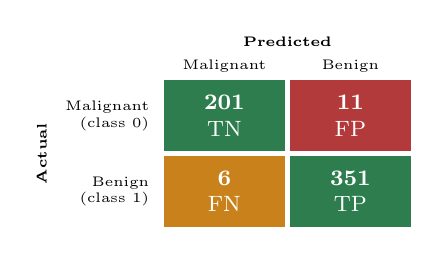
\begin{tikzpicture}[x=16mm,y=9.6mm, cell/.style={minimum width=15.4mm, minimum height=9mm,
                          font=\footnotesize, align=center, text=white}]
        \node[cell, fill=qgreen]    at (0,0)  {\textbf{201}\\TN};
        \node[cell, fill=qred]      at (1,0)  {\textbf{11}\\FP};
        \node[cell, fill=qamber]    at (0,-1) {\textbf{6}\\FN};
        \node[cell, fill=qgreen]    at (1,-1) {\textbf{351}\\TP};
        \node[font=\tiny, anchor=east, align=right] at (-0.52,0)  {Malignant\\(class 0)};
        \node[font=\tiny, anchor=east, align=right] at (-0.52,-1) {Benign\\(class 1)};
        \node[font=\tiny] at (0,0.66) {Malignant};
        \node[font=\tiny] at (1,0.66) {Benign};
        \node[font=\tiny\bfseries] at (0.5,0.98) {Predicted};
        \node[font=\tiny\bfseries, rotate=90] at (-1.45,-0.5) {Actual};
      \end{tikzpicture}\par
      \vspace{1mm}
      \footnotesize
      Accuracy $=552/569=\mathbf{0.9701}$\\
      MCC $= 0.936$\\[1pt]
      {\scriptsize QSVM-Angle 0.9649 \quad OOF stacking 0.9649}\\[1mm]
      {\scriptsize\color{qgreen}\textbf{Exactly the same numbers as in the paper.}}
    \end{column}
    \begin{column}{0.57\textwidth}
      \centering
      {\footnotesize\bfseries WBCO, seed 42 (all nine models)}\par\vspace{1mm}
      \scriptsize
      \renewcommand{\arraystretch}{1.05}
      \begin{tabular}{@{}lcccc@{}}
        \toprule
        Model & Acc & Prec & Rec & Spec \\
        \midrule
        \rowcolor{qnavy!8} Classical RBF & 0.9663 & 0.9817 & 0.9662 & 0.9665 \\
        QSVM Angle     & \textbf{0.9693} & 0.9818 & 0.9707 & 0.9665 \\
        QSVM ZZ        & 0.9649 & \textbf{0.9930} & 0.9527 & \textbf{0.9874} \\
        QSVM Amplitude & 0.9605 & 0.9685 & 0.9707 & 0.9414 \\
        QKNN Angle     & \textbf{0.9693} & 0.9753 & 0.9775 & 0.9540 \\
        QKNN ZZ        & 0.9546 & 0.9519 & \textbf{0.9797} & 0.9079 \\
        QKNN Amplitude & 0.9634 & 0.9729 & 0.9707 & 0.9498 \\
        Hard Voting    & 0.9663 & 0.9817 & 0.9662 & 0.9665 \\
        \rowcolor{qred!8} OOF Stacking & 0.9663 & 0.9795 & 0.9685 & 0.9623 \\
        \bottomrule
      \end{tabular}\par
      \vspace{1mm}
      {\scriptsize On this one split, two quantum models are slightly ahead on WBCO --- that is why one split is not enough.}
    \end{column}
  \end{columns}
  \insimple{Their code gives the same numbers for us, so any later difference comes from fairer testing, not from a mistake on our side.}
  \note{Under the code's convention (class 1 = benign), FP = 11 means 11 malignant cases predicted benign. All 36 published WDBC values (9 models x 4 metrics) reproduce exactly, and our WBCO predictions match the stored audit predictions patient by patient. An exact McNemar test finds no significant RBF-vs-stacking difference at seed 42 (WDBC p = 0.549; WBCO p = 1.0).}
\end{frame}

\begin{frame}{Result 2 --- Average Accuracy over 10 Different Splits}
  \begin{columns}[T,onlytextwidth]
    \begin{column}{0.47\textwidth}
      \scriptsize\setlength{\tabcolsep}{3.5pt}
      \renewcommand{\arraystretch}{1.12}
      \begin{tabular}{@{}lcc@{}}
        \toprule
        Model & WDBC & WBCO \\
        \midrule
        \rowcolor{qnavy!8} \textbf{Classical RBF} & \textbf{0.9731 $\pm$ 0.0017} & \textbf{0.9690 $\pm$ 0.0013} \\
        QSVM Angle     & 0.9687 $\pm$ 0.0023 & 0.9685 $\pm$ 0.0019 \\
        QSVM ZZ        & 0.9608 $\pm$ 0.0026 & 0.9638 $\pm$ 0.0016 \\
        QSVM Amplitude & 0.9552 $\pm$ 0.0022 & 0.9612 $\pm$ 0.0012 \\
        QKNN Angle     & 0.9564 $\pm$ 0.0032 & 0.9660 $\pm$ 0.0025 \\
        QKNN ZZ        & 0.9489 $\pm$ 0.0027 & 0.9511 $\pm$ 0.0043 \\
        QKNN Amplitude & 0.9480 $\pm$ 0.0032 & 0.9625 $\pm$ 0.0012 \\
        Hard Voting    & 0.9638 $\pm$ 0.0028 & 0.9654 $\pm$ 0.0010 \\
        \rowcolor{qred!8} OOF Stacking & 0.9670 $\pm$ 0.0031 & 0.9662 $\pm$ 0.0022 \\
        \bottomrule
      \end{tabular}\par
      \vspace{2mm}
      \footnotesize The classical RBF-SVM has the \textbf{highest average} on both datasets. The quantum ensemble (stacking) is 0.0061 lower on WDBC and 0.0028 lower on WBCO.
    \end{column}
    \begin{column}{0.51\textwidth}
      \centering
      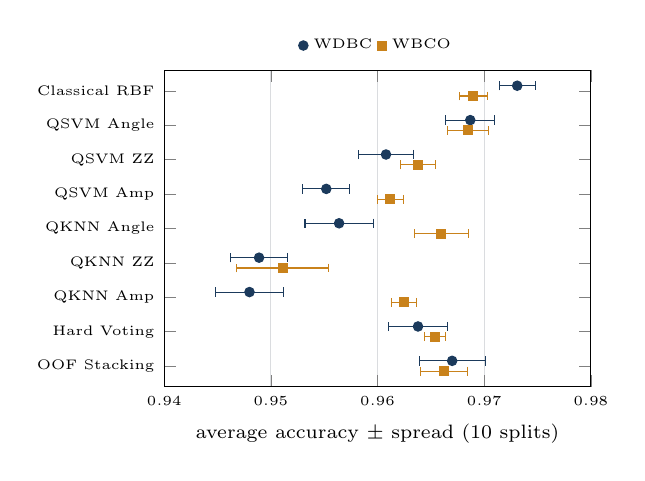
\begin{tikzpicture}
        \begin{axis}[
          width=70mm, height=56mm,
          xmin=0.940, xmax=0.980,
          ymin=0.4, ymax=9.6,
          ytick={1,...,9},
          yticklabels={OOF Stacking, Hard Voting, QKNN Amp, QKNN ZZ, QKNN Angle, QSVM Amp, QSVM ZZ, QSVM Angle, Classical RBF},
          y tick label style={font=\tiny},
          x tick label style={font=\tiny, /pgf/number format/fixed, /pgf/number format/precision=2},
          xtick={0.94,0.95,0.96,0.97,0.98},
          xlabel={\scriptsize average accuracy $\pm$ spread (10 splits)},
          xmajorgrids, grid style={qgray!25},
          legend style={font=\tiny, at={(0.5,1.02)}, anchor=south, legend columns=2, draw=none},
          ]
          \addplot+[only marks, mark=*, mark size=1.7pt, color=qnavy, mark options={fill=qnavy},
                    error bars/.cd, x dir=both, x explicit]
            coordinates {(0.9731,9.15)+-(0.0017,0) (0.9687,8.15)+-(0.0023,0) (0.9608,7.15)+-(0.0026,0)
                         (0.9552,6.15)+-(0.0022,0) (0.9564,5.15)+-(0.0032,0) (0.9489,4.15)+-(0.0027,0)
                         (0.9480,3.15)+-(0.0032,0) (0.9638,2.15)+-(0.0028,0) (0.9670,1.15)+-(0.0031,0)};
          \addplot+[only marks, mark=square*, mark size=1.6pt, color=qamber, mark options={fill=qamber},
                    error bars/.cd, x dir=both, x explicit]
            coordinates {(0.9690,8.85)+-(0.0013,0) (0.9685,7.85)+-(0.0019,0) (0.9638,6.85)+-(0.0016,0)
                         (0.9612,5.85)+-(0.0012,0) (0.9660,4.85)+-(0.0025,0) (0.9511,3.85)+-(0.0043,0)
                         (0.9625,2.85)+-(0.0012,0) (0.9654,1.85)+-(0.0010,0) (0.9662,0.85)+-(0.0022,0)};
          \legend{WDBC, WBCO}
        \end{axis}
      \end{tikzpicture}
    \end{column}
  \end{columns}
  \insimple{On average over 10 splits, the plain classical model is the best on both datasets.}
\end{frame}

\begin{frame}{Result 3 --- Classical vs.\ Quantum Ensemble, Split by Split}
  \begin{columns}[T,onlytextwidth]
    \begin{column}{0.46\textwidth}
      \centering
      {\footnotesize\bfseries WBCO, seed by seed}\par\vspace{1mm}
      \scriptsize
      \renewcommand{\arraystretch}{0.98}
      \begin{tabular}{@{}cccl@{}}
        \toprule
        Seed & RBF & Stacking & Outcome \\
        \midrule
        0   & 0.9693 & 0.9634 & \textcolor{qnavy}{\textbf{RBF} (+4)} \\
        1   & 0.9693 & 0.9678 & \textcolor{qnavy}{\textbf{RBF} (+1)} \\
        2   & 0.9693 & 0.9678 & \textcolor{qnavy}{\textbf{RBF} (+1)} \\
        3   & 0.9678 & 0.9649 & \textcolor{qnavy}{\textbf{RBF} (+2)} \\
        4   & 0.9707 & 0.9663 & \textcolor{qnavy}{\textbf{RBF} (+3)} \\
        5   & 0.9693 & 0.9619 & \textcolor{qnavy}{\textbf{RBF} (+5)} \\
        10  & 0.9678 & 0.9678 & \textcolor{qgray}{Tie} \\
        42  & 0.9663 & 0.9663 & \textcolor{qgray}{Tie} \\
        100 & 0.9693 & 0.9693 & \textcolor{qgray}{Tie} \\
        999 & 0.9707 & 0.9663 & \textcolor{qnavy}{\textbf{RBF} (+3)} \\
        \midrule
        \multicolumn{4}{c}{\textbf{7 wins / 3 ties / 0 losses for RBF}}\\
        \bottomrule
      \end{tabular}\par
      {\tiny $(+k)$ = extra patients RBF classifies correctly, out of 683. A tie means equal accuracy; the two models still disagree on 2--6 patients.\par}
    \end{column}
    \begin{column}{0.52\textwidth}
      \begin{block}{WDBC}
        \footnotesize RBF wins \textbf{all 10} splits.\\
        RBF's \emph{worst} split (0.9701) is as good as the ensemble's \emph{best} (0.9701).
      \end{block}
      \begin{block}{WBCO}
        \footnotesize RBF wins 7, ties 3 (seeds 10, 42, 100), loses 0.\\ Ranges: RBF 0.9663--0.9707; ensemble 0.9619--0.9693.
      \end{block}
      \begin{alertblock}{Together}
        \footnotesize\textbf{20 matches --- the quantum ensemble never wins.}
      \end{alertblock}
    \end{column}
  \end{columns}
  \insimple{In 20 one-to-one matches, the quantum ensemble never beat the classical model.}
  \note{The (+k) values are the accuracy differences multiplied by 683, i.e. how many more patients RBF classified correctly at that seed.}
\end{frame}

\begin{frame}{Result 4 --- After Removing Lucky Wins (Holm, 32 Tests)}
  \begin{columns}[T,onlytextwidth]
    \begin{column}{0.36\textwidth}
      \centering
      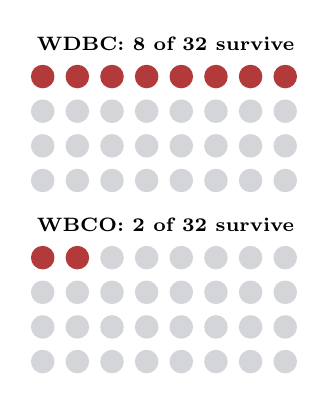
\begin{tikzpicture}[x=4.4mm,y=4.4mm]
        \node[font=\scriptsize\bfseries, anchor=west] at (-0.45,0.95) {WDBC: 8 of 32 survive};
        \foreach \k in {0,...,31}{
          \pgfmathtruncatemacro{\col}{mod(\k,8)}
          \pgfmathtruncatemacro{\row}{div(\k,8)}
          \ifnum\k<8 \def\dotcol{qred}\else\def\dotcol{qgray!30}\fi
          \fill[\dotcol] (\col,-\row) circle (0.34);
        }
        \begin{scope}[yshift=-23mm]
          \node[font=\scriptsize\bfseries, anchor=west] at (-0.45,0.95) {WBCO: 2 of 32 survive};
          \foreach \k in {0,...,31}{
            \pgfmathtruncatemacro{\col}{mod(\k,8)}
            \pgfmathtruncatemacro{\row}{div(\k,8)}
            \ifnum\k<2 \def\dotcol{qred}\else\def\dotcol{qgray!30}\fi
            \fill[\dotcol] (\col,-\row) circle (0.34);
          }
        \end{scope}
      \end{tikzpicture}\par
      \vspace{1mm}{\tiny Each dot = one test (one model, one measure, vs.\ RBF). $B=10{,}000$ re-samples.\par}
    \end{column}
    \begin{column}{0.62\textwidth}
      \scriptsize
      \renewcommand{\arraystretch}{1.05}
      \begin{tabular}{@{}llll@{}}
        \toprule
        Data & Model & Measure(s) & Result (Holm $p$) \\
        \midrule
        WDBC & QSVM-Amp   & Prec., Spec. & \textcolor{qred}{Quantum worse} (0.006) \\
        WDBC & QKNN-ZZ    & Prec., Spec. & \textcolor{qred}{Quantum worse} (0.006) \\
        WDBC & QKNN-Amp   & Prec., Spec. & \textcolor{qred}{Quantum worse} (0.028) \\
        WDBC & QKNN-Angle & Prec., Spec. & \textcolor{qred}{Quantum worse} (0.028, 0.035) \\
        \midrule
        WBCO & QKNN-ZZ    & Prec., Spec. & \textcolor{qred}{Quantum worse} (0.006) \\
        \bottomrule
      \end{tabular}\par
      \vspace{1mm}
      {\tiny\tikz\fill[qred] (0,0) circle (1.6pt); quantum worse \quad \tikz\fill[qgray!30] (0,0) circle (1.6pt); no real difference \quad (no test showed quantum better)\par}
      \vspace{0.5mm}
      {\tiny 32 = 8 models $\times$ 4 measures, each compared with RBF. Worse specificity = more cancers missed.\par}
      \vspace{1.5mm}
      \begin{alertblock}{And the quantum ensemble?}
        \footnotesize Accuracy: WDBC $p=0.45$ before correction, $1.0$ after; WBCO $p=1.0$
        $\Rightarrow$ \textbf{no advantage at all.}
      \end{alertblock}
    \end{column}
  \end{columns}
  \insimple{After removing lucky results: zero quantum wins, 10 classical wins, and no advantage for the quantum team.}
  \note{An earlier version (B = 1,000 re-samples, p allowed to be 0) showed one "quantum better" result: QKNN-Angle recall on WBCO. That was luck in the re-sampling: with bootstrap seed 42 not one of the 1,000 re-samples reversed the gap. With other seeds, or with 10,000 re-samples, its raw p is about 0.013 and its Holm p about 0.36 -- not significant. The underlying difference is 5 benign patients (exact McNemar p = 0.0625 before any correction). Source: audit_results/v3_corrections/.}
\end{frame}

\begin{frame}{Result 5 --- Is the Model Choice Really ``Adaptive''?}
  \begin{columns}[T,onlytextwidth]
    \begin{column}{0.53\textwidth}
      \centering
      {\footnotesize\bfseries WBCO, validation-accuracy criterion (paper Fig.~4)}\par
      {\tiny A fair procedure tried all 15 ways to pick 4 of the 6 models, in every fold.\par}\vspace{1mm}
      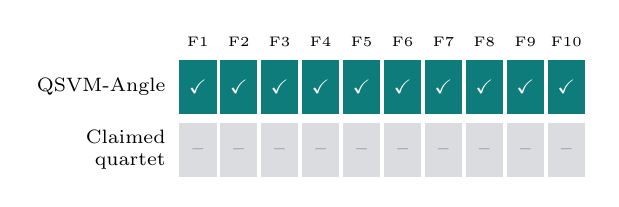
\begin{tikzpicture}[x=5.2mm,y=8mm]
        \foreach \f in {1,...,10}{
          \node[font=\tiny] at (\f,0.72) {F\f};
          \node[draw=white, fill=qteal, minimum width=4.9mm, minimum height=7mm,
                text=white, font=\scriptsize] at (\f,0) {$\checkmark$};
          \node[draw=white, fill=qgray!25, minimum width=4.9mm, minimum height=7mm,
                text=qgray, font=\scriptsize] at (\f,-1) {--};
        }
        \node[font=\scriptsize, anchor=east] at (0.45,0) {QSVM-Angle};
        \node[font=\scriptsize, anchor=east, align=right] at (0.45,-1) {Claimed\\quartet};
      \end{tikzpicture}\par
      \vspace{1mm}
      {\tiny Teal = chosen in that fold; grey = not chosen.\par}
    \end{column}
    \begin{column}{0.45\textwidth}
      \scriptsize\setlength{\tabcolsep}{4pt}
      \renewcommand{\arraystretch}{1.15}
      \begin{tabular}{@{}lcccc@{}}
        \toprule
        & \multicolumn{2}{c}{WDBC} & \multicolumn{2}{c}{WBCO}\\
        \cmidrule(lr){2-3}\cmidrule(lr){4-5}
        Criterion & Angle & Quartet & Angle & Quartet \\
        \midrule
        Validation acc. & 10/10 & 0/10 & 10/10 & 0/10 \\
        Balanced acc.   & 10/10 & 0/10 & 10/10 & 0/10 \\
        Meta-CV acc.    & 8/10  & 1/10 & 9/10  & 1/10 \\
        \bottomrule
      \end{tabular}\par
      \vspace{1mm}
      {\tiny ``Angle'': folds where QSVM-Angle is chosen. ``Quartet'': folds where the paper's four models are chosen.\par}
    \end{column}
  \end{columns}
  \vspace{3mm}
  \begin{alertblock}{Not adaptive --- fixed in advance}
    \footnotesize The fair procedure picks QSVM-Angle in 8--10 of 10 folds --- the exact model the paper left out. The paper's four are chosen in at most 1 fold. But the accuracy change is small and not significant (WDBC: 0.9684 vs.\ 0.9649, $p=0.58$).
  \end{alertblock}
  \insimple{If the choice were really automatic, it would almost always have picked QSVM-Angle --- though it would not have changed accuracy much.}
  \note{The authors say they chose the four models for diversity (two SVMs and two KNNs across encodings), which an unconstrained accuracy search does not enforce. So the fair claim is: the quartet is fixed in advance, not adaptive, and it leaves out the strongest model; it is not shown to hurt accuracy. In the single WDBC meta-CV fold that picks the paper's quartet, the score is an exact tie with another subset and the test predictions are identical.}
\end{frame}

\begin{frame}{Result 6 --- The Noise Test Used Different Circuits}
  \begin{columns}[T,onlytextwidth]
    \begin{column}{0.49\textwidth}
      \begin{block}{What the noise code really does}
        \footnotesize
        \begin{itemize}\setlength{\itemsep}{2pt}
          \item Simulates noise \textbf{correctly} with density matrices (\texttt{default.mixed}); probabilities still add up to 1
          \item But the circuits are \textbf{not the benchmarked ones}: Angle uses $R_Y$ (not $R_X$); ZZ links only \textbf{7} neighbouring pairs instead of all \textbf{28}
          \item That removes \textbf{75\%} of the entangling gates (14 instead of 56) --- the gates that suffer most from noise
        \end{itemize}
      \end{block}
      \scriptsize\setlength{\tabcolsep}{3pt}
      \begin{tabular}{@{}lcc@{}}
        \toprule
        ZZ self-similarity $K_{ii}$ (ideal $=1$) & 5\% noise & 10\% noise \\
        \midrule
        Their 7-pair circuit      & 0.19--0.23 & 0.05--0.07 \\
        Benchmarked 28-pair circuit & 0.010--0.016 & 0.004--0.005 \\
        \bottomrule
      \end{tabular}
    \end{column}
    \begin{column}{0.49\textwidth}
      \centering
      {\footnotesize\bfseries Cancer detection (specificity), 60 patients\par}\vspace{1mm}
      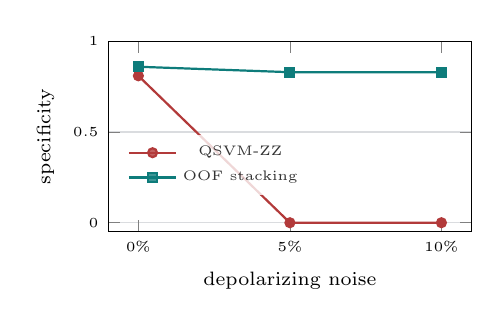
\begin{tikzpicture}
        \begin{axis}[width=62mm, height=40mm, ymin=-0.05, ymax=1.0,
          xtick={0,0.05,0.10}, xticklabels={0\%,5\%,10\%},
          x tick label style={font=\tiny}, y tick label style={font=\tiny},
          xlabel={\scriptsize depolarizing noise}, ylabel={\scriptsize specificity},
          legend style={font=\tiny, at={(0.03,0.35)}, anchor=west, draw=none, fill=white, fill opacity=0.8},
          ymajorgrids, grid style={qgray!25}]
          \addplot[qred, thick, mark=*, mark size=1.6pt] coordinates {(0,0.81)(0.05,0.0)(0.10,0.0)};
          \addplot[qteal, thick, mark=square*, mark size=1.6pt] coordinates {(0,0.86)(0.05,0.83)(0.10,0.83)};
          \legend{QSVM-ZZ, OOF stacking}
        \end{axis}
      \end{tikzpicture}\par
      \footnotesize
      With noise, QSVM-ZZ calls \textbf{every} patient benign (finds 0\% of cancers). The ensemble looks stable only because the ``manager'' sets that model's weight to $\approx 0$.
    \end{column}
  \end{columns}
  \insimple{The noise test checked an easier circuit than the one used for the main results, and the ensemble ``survives'' by silently ignoring the model that broke.}
  \note{Numbers from audit_results/noise_nisq/. The QSVM-ZZ collapse to a single class happens with both the released and the corrected circuits, at 5\% and 10\% noise. The meta-learner coefficient on QSVM-ZZ falls from 0.77-2.17 (clean) to below 0.001 in every noisy fold. This is a 60-patient simulation without shot noise, not a hardware test.}
\end{frame}

\begin{frame}{Result 7 --- Two More Code Checks}
  \begin{columns}[T,onlytextwidth]
    \begin{column}{0.49\textwidth}
      \begin{block}{A fair classical opponent (WDBC, seed 42)}
        \scriptsize\setlength{\tabcolsep}{3pt}
        \begin{tabular}{@{}lcc@{}}
          \toprule
          Model & Acc. & McNemar $p$ \\
          \midrule
          RBF-SVM, default (theirs) & 0.9701 & 0.549 \\
          RBF-SVM, tuned & \textbf{0.9719} & 0.424 \\
          XGBoost, tuned & 0.9649 & 1.000 \\
          Classical stacking, tuned & 0.9684 & 0.688 \\
          \rowcolor{qred!8} Quantum stacking & 0.9649 & --- \\
          \bottomrule
        \end{tabular}\par
        \vspace{1mm}
        \footnotesize McNemar $p$ is against the quantum stacking. Tuning (grid search) makes the classical RBF a little \textbf{better}.
      \end{block}
    \end{column}
    \begin{column}{0.49\textwidth}
      \begin{block}{The ``barren plateau'' was a bug}
        \footnotesize
        The paper says its quantum neural network (VQC, 48 weights) could not learn because of a \textbf{barren plateau}.\\[3pt]
        In the code, predictions are kept in a Python \textbf{list}, which cuts the automatic-gradient chain:
        \begin{itemize}\setlength{\itemsep}{1pt}
          \item Their loss: gradient \textbf{exactly 0} (0 of 48 non-zero)
          \item True gradient (finite differences): not zero (up to 0.092)
          \item One-line fix (\texttt{pnp.stack}): gradient restored, 48 of 48 non-zero
        \end{itemize}
      \end{block}
    \end{column}
  \end{columns}
  \insimple{The classical model was not handicapped much, and the quantum network failed because of a coding bug, not physics.}
  \note{Tuned grid for RBF: C in {0.1, 1, 10, 100}, gamma in {scale, auto, 0.01, 0.1, 1}, inner 5-fold GridSearchCV. Sources: audit_results/classical_fairness/ and audit_results/vqc_loss_bug_gradient_audit.csv. The fixed gradient matches finite differences to about 1e-11.}
\end{frame}

\begin{frame}{Result 8 --- Can We Trust the Probabilities? (WDBC)}
  \begin{columns}[T,onlytextwidth]
    \begin{column}{0.50\textwidth}
      \footnotesize
      \renewcommand{\arraystretch}{1.2}
      \begin{tabular}{@{}lcc@{}}
        \toprule
        Model & ECE $\downarrow$ & Brier $\downarrow$ \\
        \midrule
        Classical RBF-SVM            & \textbf{0.0173} & \textbf{0.0233} \\
        RBF-SVM + Platt scaling      & 0.0419 & 0.0260 \\
        OOF stacking (raw)           & \textcolor{qred}{0.0332} & \textcolor{qred}{0.0299} \\
        OOF stacking + Platt scaling & 0.0267 & 0.0290 \\
        \bottomrule
      \end{tabular}\par
      \vspace{2mm}
      \scriptsize
      \begin{itemize}\setlength{\itemsep}{1pt}
        \item \textbf{ECE}: if it says ``90\% sure'', is it right 90\% of the time?
        \item \textbf{Brier}: average error of the probabilities
        \item \textbf{Platt scaling}: a simple fix that re-scales them
      \end{itemize}
    \end{column}
    \begin{column}{0.48\textwidth}
      \centering
      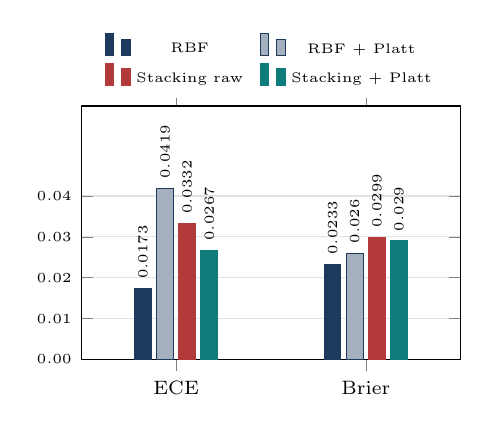
\begin{tikzpicture}
        \begin{axis}[ybar, width=64mm, height=48mm, bar width=6pt,
          symbolic x coords={ECE,Brier}, xtick=data, enlarge x limits=0.5,
          ymin=0, ymax=0.062, scaled y ticks=false,
          ytick={0,0.01,0.02,0.03,0.04},
          yticklabel style={font=\tiny, /pgf/number format/fixed, /pgf/number format/precision=2, /pgf/number format/fixed zerofill},
          x tick label style={font=\scriptsize},
          nodes near coords={\pgfmathprintnumber[fixed,precision=4]{\pgfplotspointmeta}},
          nodes near coords style={font=\tiny, rotate=90, anchor=west},
          legend style={font=\tiny, at={(0.5,1.03)}, anchor=south, legend columns=2, draw=none,
                        /tikz/every even column/.append style={column sep=4pt}},
          ymajorgrids, grid style={qgray!20}]
          \addplot[fill=qnavy, draw=qnavy] coordinates {(ECE,0.0173) (Brier,0.0233)};
          \addplot[fill=qnavy!40, draw=qnavy] coordinates {(ECE,0.0419) (Brier,0.0260)};
          \addplot[fill=qred,  draw=qred]  coordinates {(ECE,0.0332) (Brier,0.0299)};
          \addplot[fill=qteal, draw=qteal] coordinates {(ECE,0.0267) (Brier,0.0290)};
          \legend{RBF, RBF + Platt, Stacking raw, Stacking + Platt}
        \end{axis}
      \end{tikzpicture}
    \end{column}
  \end{columns}
  \vspace{1mm}
  {\footnotesize The raw classical RBF has the best probabilities on both measures. Platt scaling helps the ensemble a little but not enough to catch up.\par}
  \insimple{The classical model's ``how sure am I'' numbers are the most trustworthy.}
  \note{Source: audit_results/calibration/ (10 equal-width bins, seed 42). RBF probabilities come from LIBSVM's built-in Platt fit; adding a second Platt step on top makes RBF worse.}
\end{frame}

\begin{frame}{Result 9 --- Do the Findings Hold on the Second Dataset?}
  \centering\scriptsize
  \renewcommand{\arraystretch}{1.05}
  \begin{tabular}{@{}c L{46mm} L{60mm} c@{}}
    \toprule
    \# & What we found on WDBC & What we found on WBCO & Verdict \\
    \midrule
    1 & 10 splits: RBF wins all 10 & RBF wins 7, ties 3, loses 0 & \verdict{qamber}{Partially confirmed} \\
    2 & Holm (32 tests): 8 left, all ``quantum worse'' & 2 left, both ``quantum worse''; no ensemble advantage & \verdict{qgreen}{Confirmed} \\
    3 & Fold-local vs.\ global preparation: equivalent ($p=0.039$) & Equivalent ($p=0.0004$) & \verdict{qgreen}{Confirmed} \\
    4 & Model choice: QSVM-Angle 8--10/10 folds; paper's four $\le$1/10 & QSVM-Angle 9--10/10; paper's four $\le$1/10 & \verdict{qgreen}{Confirmed} \\
    \bottomrule
  \end{tabular}\par
  \vspace{2mm}
  \begin{exampleblock}{Second dataset, 10 splits}
    \footnotesize The classical RBF is still the best on average (0.9690), QSVM-Angle just behind (0.9685). QKNN-ZZ changes most between splits ($\sigma=0.0043$).
  \end{exampleblock}
  \insimple{On the second dataset, three findings hold fully and the seed result holds in part (ties instead of wins).}
  \note{Verdicts follow Table X of the v3 paper.}
\end{frame}

% =====================================================================
\renewcommand{\secquestion}{Where could we be wrong?}
\section{Threats to Validity}
% =====================================================================

\begin{frame}{Limits of Our Audit}
  \begin{columns}[T,onlytextwidth]
    \begin{column}{0.49\textwidth}
      \begin{block}{Inside the study (internal)}
        \footnotesize We used their released code; other versions of PennyLane or scikit-learn might behave slightly differently. 10 splits are many, but not all possible splits.
      \end{block}
      \begin{block}{What we measured (construct)}
        \footnotesize We compared splits mainly by accuracy; the Holm check covers four measures. In the code, ``recall'' means benign detection and ``specificity'' means cancer detection. A real clinical tool would also need checks of calibration and fairness.
      \end{block}
    \end{column}
    \begin{column}{0.49\textwidth}
      \begin{block}{Other data and hardware (external)}
        \footnotesize Both datasets are small, clean tables (37\% / 35\% cancer). Images or real quantum computers may give different results.
      \end{block}
      \begin{block}{The statistics}
        \footnotesize The bootstrap assumes patients are roughly independent --- reasonable here. Bootstrap results move a little with the random seed, so we use 10,000 re-samples. Holm is strict on purpose: for medical claims, avoiding any false win matters most.
      \end{block}
    \end{column}
  \end{columns}
  \insimple{Our answer is about this method, on these datasets, in simulation --- not about quantum computing in general.}
\end{frame}

% =====================================================================
\renewcommand{\secquestion}{What should the field take away?}
\section{Conclusion}
% =====================================================================

\begin{frame}{Six Key Findings}
  \small
  \begin{enumerate}\setlength{\itemsep}{2pt}
    \item \textbf{Same numbers:} we got exactly their seed-42 results.
    \item \textbf{Many splits:} the classical RBF-SVM equals or beats the quantum ensemble in \textbf{20 of 20} matches --- it never loses.
    \item \textbf{Removing lucky wins:} no quantum win on either dataset; every surviving test shows a quantum model missing more cancers; the ensemble has no advantage.
    \item \textbf{Model choice:} a fair procedure picks QSVM-Angle, the model the paper left out, in 8--10 of 10 folds; the paper's four are chosen at most once.
    \item \textbf{Noise:} the noise test used simpler circuits than the main results (75\% fewer entangling gates), so the ``robust to noise'' claim does not apply to the benchmarked models.
    \item \textbf{Barren plateau:} the quantum network's failure was a gradient bug (gradient exactly 0), not physics.
  \end{enumerate}
  \insimple{Bottom line: the claimed quantum advantage is not supported --- test many splits, correct for luck, tune the classical model, check gradients, and test noise on the same circuits.}
\end{frame}





\begin{frame}[c]
  \centering
  {\Huge\bfseries\color{qnavy} Thank you}\par\vspace{3mm}
  {\Large\color{qteal} Questions and discussion}\par\vspace{8mm}
  \begin{beamercolorbox}[wd=0.86\textwidth,sep=6pt,rounded=true,center]{simplebox}
    \small Code-level audit \textbullet\ 10 seeds $\times$ 2 datasets \textbullet\ 32 Holm-corrected hypotheses \textbullet\ nested model selection \textbullet\ noise-circuit and gradient checks
  \end{beamercolorbox}\par\vspace{6mm}
  {\small\bfseries Muhammad Wajahat\par}\vspace{1mm}
  {\footnotesize Department of Computer Science, National Biomedical Computational Center, Islamabad, Pakistan\par}
\end{frame}

\end{document}
